% 0582(본책 104쪽) — △ABC 의 외접원, BC 연장선과 접점 A 의 접선의 교점 D, ∠ADB 의 이등분선과 AB 의 교점 E, ∠BAC=50°, ∠AED 표시. 스캔 삽화를 TikZ 로 다시 그림.
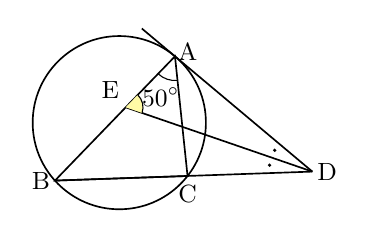
\begin{tikzpicture}[scale=1.1, line width=0.6pt]
  \draw (0.000,0.000) circle (1.000);
  \draw (0.643,0.766) -- (-0.743,-0.669) -- (0.788,-0.616) -- cycle;
  \draw (-0.743,-0.669) -- (2.229,-0.565);
  \draw (2.229,-0.565) -- (0.260,1.087);
  \draw (2.229,-0.565) -- (0.074,0.177);
  \draw[line width=0.4pt] (0.448,0.565) arc[start angle=-134.000, end angle=-84.000, radius=0.280];
  \node[font=\small, inner sep=1pt] at (0.480,0.293) {$50^\circ$};
  \fill[yellow!35] (0.074,0.177) -- ++(-19.000:0.200) arc[start angle=-19.000, end angle=46.000, radius=0.200] -- cycle;
  \draw[line width=0.4pt] (0.263,0.112) arc[start angle=-19.000, end angle=46.000, radius=0.200];
  \fill (1.735,-0.491) circle (0.6pt);
  \fill (1.794,-0.319) circle (0.6pt);
  \node[font=\small, anchor=west, inner sep=1.5pt] at (0.623,0.816) {A};
  \node[font=\small, anchor=east, inner sep=1.5pt] at (-0.743,-0.669) {B};
  \node[font=\small, anchor=north, inner sep=1.5pt] at (0.788,-0.666) {C};
  \node[font=\small, anchor=west, inner sep=1.5pt] at (2.229,-0.565) {D};
  \node[font=\small, anchor=south east, inner sep=1.5pt] at (0.054,0.227) {E};
\end{tikzpicture}
